% Бүлэг 1

\chapter{Прокси дахин шифрлэлтэд суурилсан файл хуваалцах систем хөгжүүлэх}

\label{Chapter3} % Энэ бүлэг рүү ишлэл хийх бол \ref{Chapter1} командыг ашигла 
\pagecolor{white}

%-------------------------------------------------------------------------------
%	SECTION 1
%-------------------------------------------------------------------------------
\section{Системийн шаардлага}
Систем нь түлхүүр үүсгэх файл хадгалах сервер, өгөгдөл эзэмшигч, өгөгдөл хэрэглэгч гэсэн үндсэн гурван хэсгээс тогтоно. Өгөгдөл эзэмшигч бүртгэл үүсгэж өөрийн нийтийн түлхүүр болон хувийн түлхүүрийг үүсгэж авна. Файл шифрлэх болон тайлах үйлдэлийг өөрийн төхөөрөмж дээр үйлдэнэ.

\textbf{Системийн оролцогч}
\begin{itemize}
    \item Хэрлэгч
\end{itemize}

\textbf{Системийн тоглогч}
\begin{itemize}
    \item Өгөгдөл эзэмшигч
    \item Өгөгдөл хэрэглэгч
\end{itemize}

\subsection*{Функцийн шаардлага}
Өгөгдөл эзэмшигчийн функционал шаардлага:
\begin{itemize}
    \item Системд өөрийн бүртгэлийг үүсгэх
    \item Файл оруулах, шифрлэх
    \item Файлыг тайлах хэрлэгч сонгох
    \item Шифрлсэн файлыг хуваалцсан хэрлэгчдийн жагсаалт
\end{itemize}
Өгөгдөл хэрэглэгчийн функционал шаардлага:
\begin{itemize}
    \item Системд өөрийн бүртгэлийг үүсгэх
    \item Өөрт хуваацлсан файлын жагсаалт
    \item Файлыг татаж авах
    \item Шифрлсэн файлыг тайлах
\end{itemize}

\subsection*{Функцийн бус шаардлага}
\begin{enumerate}
    \item Файлыг шифрлэх, шифрийг тайлах хурдан гүйцэтгэдэг байх
    \item Хэрэглэгчийн интерфэйс ойлгомжтой энгийн байх.
    \item Прокси серверт файлыг шифрлсэн байдлаар хадгалах, хуваалцах
    \item Өөрийн бүртгэлийг ашиглаж нэвтрэх
    \item Хувийн түлхүүрийг хэрлэгчийн төхөөрөмж дээр авч явах
\end{enumerate}

\subsection*{Юзкейс диаграмм}
Системийн хэрлэгчид ямар үйлдлүүдийг системд хийж болохыг харуулсан хэрэглээний диаграммыг харууллаа.
\begin{figure}[ht]
    \centering
    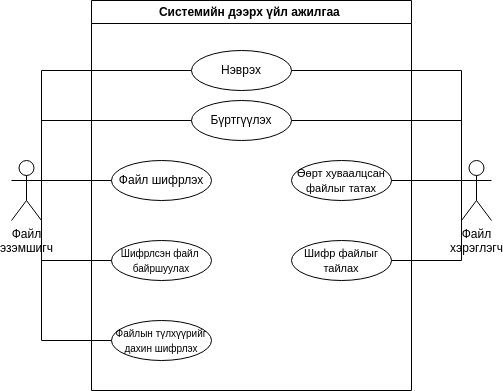
\includegraphics[scale=0.6]{Figures/usecase.drawio.png}
    \caption[Usecase diagram]{Юзкейс диаграмм}
    \label{fig:usecase}
\end{figure}
\subsection*{Юзкейс тодорхойлолт}

\begin{table}
    \caption{Бүртгүүлэх юзкейсийн тодорхойлолт}
    \label{tab:treatments}
    \footnotesize
    \centering
    \begin{tabularx}{\textwidth}{|>{\hsize=0.3\hsize}X|>{\hsize=0.7\hsize}X|}
        \hline
        \multicolumn{2}{|c|}{Бүртгүүлэх} \\
        \hline
        ID & 1 \\
        \hline
        Тодорхойлолт & \\
        \hline
        Өмнөх нөхцөл & \\
        \hline
        Үндсэн урсгал & \\
        \hline
        Дараах нөхцөл & \\
        \hline
      \end{tabularx}
\end{table}

\begin{table}
    \caption{Нэвтрэх юзкейсийн тодорхойлолт}
    \label{tab:treatments}
    \footnotesize
    \centering
    \begin{tabularx}{\textwidth}{|>{\hsize=0.3\hsize}X|>{\hsize=0.7\hsize}X|}
        \hline
        \multicolumn{2}{|c|}{Нэвтрэх} \\
        \hline
        ID & 2 \\
        \hline
        Тодорхойлолт & \\
        \hline
        Өмнөх нөхцөл & \\
        \hline
        Үндсэн урсгал & \\
        \hline
        Дараах нөхцөл & \\
        \hline
      \end{tabularx}
\end{table}

\begin{table}
    \caption{Файл шифрлэх юзкейсийн тодорхойлолт}
    \label{tab:treatments}
    \footnotesize
    \centering
    \begin{tabularx}{\textwidth}{|>{\hsize=0.3\hsize}X|>{\hsize=0.7\hsize}X|}
        \hline
        \multicolumn{2}{|c|}{Файл шифрлэх} \\
        \hline
        ID & 3 \\
        \hline
        Тодорхойлолт & \\
        \hline
        Өмнөх нөхцөл & \\
        \hline
        Үндсэн урсгал & \\
        \hline
        Дараах нөхцөл & \\
        \hline
      \end{tabularx}
\end{table}

\begin{table}
    \caption{Шифрлсэн файл серверт байршуулах юзкейсийн тодорхойлолт}
    \label{tab:treatments}
    \footnotesize
    \centering
    \begin{tabularx}{\textwidth}{|>{\hsize=0.3\hsize}X|>{\hsize=0.7\hsize}X|}
        \hline
        \multicolumn{2}{|c|}{Шифрлсэн файл серверт байршуулах} \\
        \hline
        ID & 4 \\
        \hline
        Тодорхойлолт & \\
        \hline
        Өмнөх нөхцөл & \\
        \hline
        Үндсэн урсгал & \\
        \hline
        Дараах нөхцөл & \\
        \hline
      \end{tabularx}
\end{table}

\begin{table}
    \caption{Файл хуваалцах тодорхойлолт}
    \label{tab:treatments}
    \footnotesize
    \centering
    \begin{tabularx}{\textwidth}{|>{\hsize=0.3\hsize}X|>{\hsize=0.7\hsize}X|}
        \hline
        \multicolumn{2}{|c|}{Файл хуваалцах} \\
        \hline
        ID & 5 \\
        \hline
        Тодорхойлолт & \\
        \hline
        Өмнөх нөхцөл & \\
        \hline
        Үндсэн урсгал & \\
        \hline
        Дараах нөхцөл & \\
        \hline
      \end{tabularx}
\end{table}

\begin{table}
    \caption{Файл татах тодорхойлолт}
    \label{tab:treatments}
    \footnotesize
    \centering
    \begin{tabularx}{\textwidth}{|>{\hsize=0.3\hsize}X|>{\hsize=0.7\hsize}X|}
        \hline
        \multicolumn{2}{|c|}{Файл татах} \\
        \hline
        ID & 6 \\
        \hline
        Тодорхойлолт & \\
        \hline
        Өмнөх нөхцөл & \\
        \hline
        Үндсэн урсгал & \\
        \hline
        Дараах нөхцөл & \\
        \hline
      \end{tabularx}
\end{table}

\begin{table}
    \caption{Шифрлсэн файлын тайлах юзкейсийн тодорхойлолт}
    \label{tab:treatments}
    \footnotesize
    \centering
    \begin{tabularx}{\textwidth}{|>{\hsize=0.3\hsize}X|>{\hsize=0.7\hsize}X|}
        \hline
        \multicolumn{2}{|c|}{Шифрлсэн файлын тайлах} \\
        \hline
        ID & 7 \\
        \hline
        Тодорхойлолт & \\
        \hline
        Өмнөх нөхцөл & \\
        \hline
        Үндсэн урсгал & \\
        \hline
        Дараах нөхцөл & \\
        \hline
      \end{tabularx}
\end{table}

%-------------------------------------------------------------------------------
%	SECTION 2
%-------------------------------------------------------------------------------
\section{Системийн загвар}

\subsection*{Үйл ажилгааны диаграмм}

\subsection*{Өгөгдлийн сангийн бүтэц}

%-------------------------------------------------------------------------------
%	SECTION 3
%-------------------------------------------------------------------------------
\section{Системийн хөгжүүлэх}

%-------------------------------------------------------------------------------
%	SECTION 4
%-------------------------------------------------------------------------------
\section{Файл хуваалцах системийг турших}
%-------------------------------------------------------------------------------
%	SECTION 5
%-------------------------------------------------------------------------------

\section{Дүгнэлт}

